\documentclass{article}
\usepackage{amsmath}
\usepackage{amsfonts}
\usepackage{blindtext}
\usepackage{graphicx}
\graphicspath{ {./} }
\begin{document}

\section{Foreword}
Author : Anderson Chau
\newline 
\newline 
Disclaimer : The notes are written only for my understanding and memorization purpose after I have self-studied those online lecture notes. 
% ######################################################################
% ######################################################################
% ######################################################################

\section{Main Idea}
The old trick : (i) Forward feed (ii) Compute Loss ( NN output vs training data ) (iii) Backpropagation with Gradient Descent to tune parameters \newline 
2. Use activation functions to avoid the model to be a pure linear model, which is useless (just ax+b) \newline
3.  Examples of activation functions : Signmoid , (Leaky) ReLU, tanh etc. \newline
\section{ANN Structure}
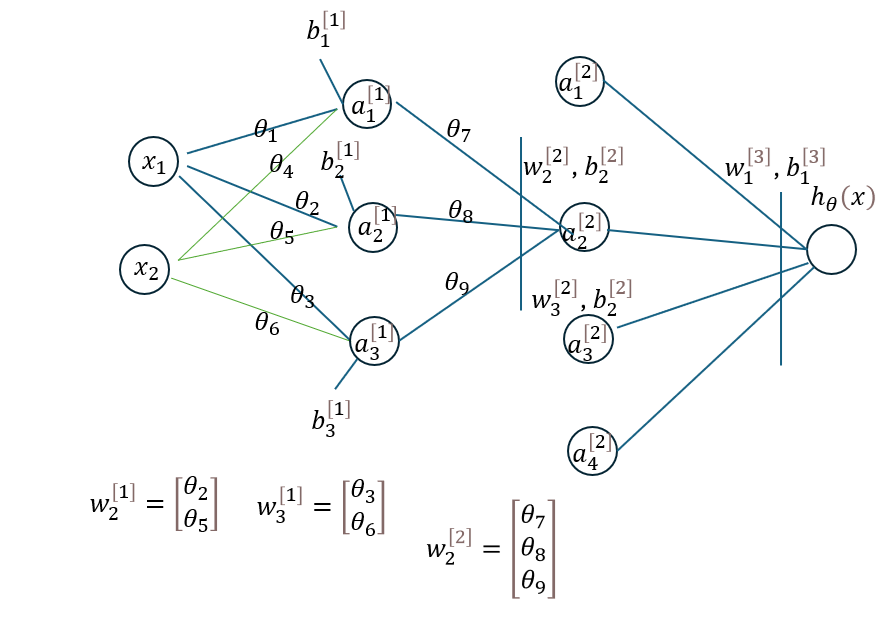
\includegraphics{diagram1}
w's and b's are parameters : Totally ther are Hidden Layer 1 (layer 1) (2x3 + 3) + Hidden Layer 1  (layer 2 ) (3x4 + 4) + Output Layer (layer 3)(4x1 +1 ) number of parameters    
\section{Forward Feed (see above NN diagram) }
\[a_1 = \text{ReLU}(\theta_1 x_1 + \theta_4 x_2 + b_{1}^{[1]})\]
\[a_2 = \text{ReLU}(\theta_2 x_1 + \theta_5 x_2 + b_{2}^{[1]})\]
Let i be \(i^{th}\) layer and j be \(j^{th}\) neuron ( count vertifically) this layer of NN \newline 
Rewriting the notation : \(w_{j}^{[i]}\) as \(\textbf{VECTOR}\) of input \(\theta\)'s for layer i and \(j^{th}\) neuron. \newline
With the above, Layer 1 of NN can be expressed as: \newline 

For all \( j \in [1, \dots, m] \): (m=3, count vertically, is the number of number of neuron layer 1 )
\[
z_j = \mathbf{w}^{[1]}_j{}^\top \mathbf{x} + b^{[1]}_j \quad \text{where} \quad \mathbf{w}^{[1]}_j \in R^d, \; b^{[1]}_j \in R
\]
(d = 2 , count vertically, is the number of number of previous layer , layer 0 )
\[
a_j = \text{ReLU}(z_j),
\]

\[
\mathbf{a} = [a_1, \dots, a_m]^\top \in R^m
\]
For Layer 3 :
\[
\bar{h}_\theta(\mathbf{x}) = \mathbf{w}^{[3]}{}^\top \mathbf{a} + b^{[3]} \quad \text{where} \quad \mathbf{w}^{[3]} \in R^n, \; b^{[3]} \in R
\] 
(n = 4, count vertically, is the number of number of neuron  layer, layer 2  )
\section{Vectorization of Forward Feeding}

Just by stacking the parameters . for layer 1 : 
\[W^{[1]} = \begin{bmatrix} - w^{[1]T}_1 - \\ - w^{[1]T}_2 - \\ \vdots \\ - w^{[1]T}_m - \end{bmatrix} \in R^{m \times d}\]

\[
\mathbf{z} = \begin{bmatrix}
z_1 \\
z_2 \\
\vdots \\
z_m
\end{bmatrix} \in \mathbb{R}^{m \times 1} =
\begin{bmatrix}
-w^{[1]T}_1- \\
-w^{[1]T}_2- \\
\vdots \\
-w^{[1]T}_m-
\end{bmatrix}
\begin{bmatrix}
x_1 \\
x_2 \\
\vdots \\
x_d
\end{bmatrix}
+
\begin{bmatrix}
b^{[1]}_1 \\
b^{[1]}_2 \\
\vdots \\
b^{[1]}_m
\end{bmatrix}
\]
Hence we get: 
\[ z^{[1]}=W^{[1]}x+b^{[1]} \]
\[ a^{[1]} = ReLU(z^{[1]}) \]
\[ z^{[2]}=W^{[2]}a^{[1]}+b^{[2]} \]
\[ a^{[2]} = ReLU(z^{[2]}) \]
\[ h=W^{[3]}a^{[2]}+b^{[3]} \]
In General : 

\[
\begin{aligned}
a^{[1]} &= \text{ReLU}(W^{[1]}x + b^{[1]}) \\
a^{[2]} &= \text{ReLU}(W^{[2]}a^{[1]} + b^{[2]}) \\
&\ \, \vdots \\
a^{[r-1]} &= \text{ReLU}(W^{[r-1]}a^{[r-2]} + b^{[r-1]}) \\
h(x) &= W^{[r]}a^{[r-1]} + b^{[r]}
\end{aligned}
\]
Also, for loss function J
\[J = (1/2)(h-o)^2\]
Some common loss function for J : Common : (1) Mean Sequared Error (2) Cross Entropy Loss 


\section{Matrix Calculus}
1. Jacobian of elementwise operation fuunction are diagonal. Therefore  \( \frac{\partial a^{[i]} }{\partial z^{[i]}} \) is a diagonal matrix \newline

\section{Vectorized Backpropagation}
Our objective is to make use of matrix calculus, gradient descent to tune W and b to minimize J by SGD or mini-batch GD \newline

Algo 1 SGD : 
 1: Hyperparameter: learning rate \(\alpha\), number of total iteration \(n_{iter}\). \newline
 2: Initialize \(\theta\) randomly. \newline
 3: for i = 1 to niter do \newline
 4: Sample j uniformly from {1,...,n}, and update \(\theta\) by \newline
\[ \theta := \theta - \alpha \nabla_\theta J^{(j)}(\theta) \] 
By Chain Rule of matrix calculus 
\[
\frac{\partial L }{\partial W_{ij}^{[2]}} = ( \frac{\partial L }{\partial a^{[3]}} \frac{\partial a^{[3]}}{\partial z^{[3]}} )
(\frac{\partial z^{[3]}}{\partial a^{[2]}}) ( \frac{\partial a^{[2]}}{\partial z^{[2]}})( \frac{\partial z^{[2]}}{\partial W_{ij}^{[2]}})
\]

\[
= [ (a^{[3]}-y)W[3] \bigodot g(z^{[2]}) ]_i a_j^{[1]T} 
\]
stacking up again :
\[
\frac{\partial L }{\partial W^{[2]}} = [ (a^{[3]}-y)W[3] \bigodot g(z^{[2]}) ] a^{[1]T} 
\]
We see here the step of GD is based on next layer's value, therefore we have update back propagated to previous layer.


\end{document}
